%% ======================================================================
%% 04d_dron_rampa_bateria.tex -- 3. Model (part 3): why a drone on the ramp and battery margin
%% Numbers: scripts_modelo/rampa.py and scripts_modelo/bateria.py
%% ======================================================================
\subsection{Why a drone on the ramp}
\label{sec:porquedron}

AeroTray's intermediate stage could have been a motorized two-axis gimbal. Using the equations derived above, this section quantifies what the octocopter contributes on the ramp and at what cost.

\paragraph{Core idea: an actuator that does not push against the base}
A plate driven by base-mounted servos, or by a motorized gimbal, generates its torque \emph{between} the base and the plate. By action and reaction, three things happen: every base tilt (both the slope and the jolts across the ramp breaks) must be subtracted out of the actuator's own stroke; those jolts reach the plate through a rigid transmission; and the level reference is the base itself. The octocopter on the spherical joint breaks that chain. The spherical joint transmits force only, not torque. The drone generates its torque against the air and references gravity with its IMU. Ground slope therefore never enters the plate, and the actuators separate by scale: the drone handles large, slow angles (the slope, \SIrange{0}{20}{\degree}, below \SI{0.3}{\hertz}), while the servos handle the small, fast angles required by the ball. No stage reacting against the base can provide this separation without consuming actuator stroke. The drone also adds an exclusive capability: its thrust acts as adjustable ballast (point~2).

\paragraph{Evidence from the 18 November logs}
Across the eleven runs recorded that day, the drone sat free on the spherical joint at \SI{1300}{\micro\second}. Mean servo stroke usage was 36--57\% over the seven ramp runs and 43--63\% over the four flat-ground runs. Median pulse-width bias on the ramp never exceeded \SI{\pm60}{\micro\second}. With the tray fixed to the base, merely leveling the \SI{10}{\degree} slope would have required a bias of about \SI{204}{\micro\second}---93\% of available stroke. The servos worked no harder on the ramp than on flat ground: the slope did not reach the plate. A direct comparative test---Test~D in Section~\ref{sec:metodologia}, traversing the same ramp with the drone locked to the base (\emph{servos only}) versus free on the joint to compare servo usage, saturation, ball error, and losses---remains future work (Section~\ref{sec:limits}).

\paragraph{1. Leveling: slope disappears from the plate}
By \eqref{eq:tilt}, absolute plate tilt is $\theta+\alpha_y$ and does not contain $\beta$. The octocopter drives $\theta$ to zero using its own IMU, so the servos only regulate ball position. With the tray fixed to the base, the slope would consume $\beta$ of the \SI{\pm10.8}{\degree} plate travel: on the \SI{10}{\degree} ramp only \SI{0.8}{\degree} would remain for ball control, and at \SI{20}{\degree} the plate could not level. In hover, the octocopter held the tray plane within 0.55--1.7$^\circ$ RMS of horizontal (Section~\ref{sec:flights}), leaving 84--95\% of the servo stroke free. A gimbal with its own IMU could also level the tray, though still reacting against the base with finite actuator stroke; the next function, however, is exclusive to the drone.

\paragraph{2. Weight relief: adjustable ballast}
Let $f=T/\big((m+m_c)g\big)\in[0,1]$ be the fraction of the module weight supported by the rotors. While $f<1$, the module rests on the lower stop of the vertical guide \eqref{eq:guide}, and because it self-levels, its thrust is vertical in $\{W\}$. In the moment balance \eqref{eq:tip}, thrust therefore reduces the effective weight of the module at the spherical joint to $(1-f)(m+m_c)$. With the rest of the robot (mass $M_b=\SI{6.8}{\kilo\gram}$, CM at $x_b=\SI{0.088}{\metre}$ ahead of the driven axle and $h_b=\SI{0.081}{\metre}$ above the support plane, deduced from the measured tip-over slopes) and $m_a=m+m_c$,
\begin{equation}
\begin{gathered}
  M(f)=M_b+(1-f)m_a,\\
  x_G(f)=\frac{M_bx_b+(1-f)m_a\ell_J}{M(f)},\qquad
  h_G(f)=\frac{M_bh_b+(1-f)m_a(h_{J0}+d)}{M(f)},
\end{gathered}
  \label{eq:descarga}
\end{equation}
and substituting \eqref{eq:descarga} into the static condition of \eqref{eq:tip}, \eqref{eq:vss}, and the traction condition of Section~\ref{sec:basedyn} gives the relieved limits. The acceleration margin requires one extra distinction: thrust removes \emph{weight}, not \emph{mass}. The vertical guide still accelerates all \SI{3.6}{\kilo\gram} of the module together with the base, so its full d'Alembert force acts at the spherical joint and
\begin{equation}
\begin{split}
  a_{\max}(f,\beta)=\frac{g}{M_bh_b+m_a(h_{J0}+d)}\Big\{&\big[M_bx_b+(1-f)m_a\ell_J\big]\cos\beta\\
  &-\big[M_bh_b+(1-f)m_a(h_{J0}+d)\big]\sin\beta\Big\}.
\end{split}
  \label{eq:amaxf}
\end{equation} Figure~\ref{fig:rampa} and Table~\ref{tab:rampa} show the outcome. The \SI{3.6}{\kilo\gram} module sits high (spherical joint at \SI{0.5}{\metre}) and nearly on the same vertical line as the CM of the rest of the robot ($\ell_J\approx x_b\approx\SI{88}{\milli\metre}$). Supporting a fraction $f$ of its weight with the rotors therefore shifts the CM neither forward nor backward: it \emph{lowers} it, improving tip-over stability in both directions.
\begin{itemize}
  \item \textbf{Tip-over.} Uphill static tip-over slope rises from \SI{21.4}{\degree} ($f=0$; measured: \SI{21.5}{\degree}) to \SI{27.7}{\degree} ($f=0.5$) and \SI{47.4}{\degree} ($f=1$). Downhill, it rises from \SI{30.5}{\degree} to \SI{38.2}{\degree} and \SI{58.5}{\degree}. On the \SI{10}{\degree} ramp, the uphill margin grows from \SI{11.5}{\degree} to \SI{17.7}{\degree} at $f=0.5$, a 54\% increase.
  \item \textbf{Acceleration margin.} At \SI{10}{\degree} it barely changes (\SI{2.1}{\metre\per\second\squared}), because thrust removes weight rather than mass \eqref{eq:amaxf}. At \SI{20}{\degree} it grows from \SI{0.26}{\metre\per\second\squared} to \SI{0.92}{\metre\per\second\squared} at $f=0.5$---a 3.5-fold increase. Weight relief becomes decisive on steep slopes.
  \item \textbf{Traction.} The friction coefficient required at the driven wheels increases modestly: from 0.25 to 0.27 at \SI{10}{\degree} and from 0.40 to 0.44 at \SI{20}{\degree} for $f=0.5$, reaching 0.52 at $f=1$. All values stay below the rubber-on-wood range (0.5--0.8). Even so, the drone should not hover on the ramp: at $f=1$, traction on a \SI{20}{\degree} slope sits at the limit.
\end{itemize}
We propose an operating window of $f=0.35$--0.55 (\emph{ramp mode}). This corresponds to a collective of 1460--\SI{1560}{\micro\second} on charged batteries---below the firmware flight threshold (\SI{1650}{\micro\second})---and 5--\SI{9}{\ampere} per branch (power scales as $f^{3/2}$). One minute of climbing draws 0.08--\SI{0.15}{\ampere\hour} per battery, or 2--5\% of capacity. On the actual test ramp (\SI{0.7}{\metre} uphill at \SI{10}{\degree}, \SI{0.8}{\metre} flat plateau, and \SI{0.7}{\metre} downhill, \SI{12.2}{\centi\metre} height; Fig.~\ref{fig:rampa_cotas}), the model predicts a full cycle at 15\% duty cycle of about \SI{41}{\second} at idle (\SI{24}{\second} climb) and \SI{37}{\second} in ramp mode (\SI{20}{\second} climb), and about \SI{19}{\second} at 25\% duty cycle (23 November tests).

\begin{figure}[!htbp]
\centering
\begin{tikzpicture}[font=\footnotesize, >=Latex]
  % True scale (1 m = 4.10 cm). Ramp measured 24 Nov: 0.7 m at 10 deg + 0.8 m + 0.7 m at 10 deg
  % Q1=(0,0), Q2=(2.826, 0.498), Q3=(6.106, 0.498), Q4=(8.932, 0)
  \coordinate (Q1) at (0.000, 0.000);
  \coordinate (Q2) at (2.826, 0.498);
  \coordinate (Q3) at (6.106, 0.498);
  \coordinate (Q4) at (8.932, 0.000);

  % Level ground (approach and exit)
  \fill[pGris!18] (-0.95,-0.20) rectangle (10.10,0.00);
  \draw[thick, pGris!80!black] (-0.95,0.00) -- (10.10,0.00);

  % Ramp profile (1:1 scale)
  \fill[pGris!10] (Q1) -- (Q2) -- (Q3) -- (Q4) -- cycle;
  \draw[very thick, pGris!85!black] (Q1) -- (Q2) -- (Q3) -- (Q4);

  % Subtle vertical dashed guides under plateau
  \draw[dashed, pGris!60] (Q2) -- (2.826,0.00);
  \draw[dashed, pGris!60] (Q3) -- (6.106,0.00);

  % 10 deg slope angles at Q1 and Q4
  \draw[pAzul, thick] (1.10,0.00) arc (0:10:1.10);
  \node[pAzul] at (1.52,0.11) {\SI{10}{\degree}};
  \draw[pAzul, thick] (7.832,0.00) arc (180:170:1.10);
  \node[pAzul] at (7.41,0.11) {\SI{10}{\degree}};

  % Vertical height dimension (12.2 cm) on the right
  \draw[dotted, pGris] (Q3) -- (9.90,0.498);
  \draw[<->, pGris!85!black] (9.75,0.00) -- (9.75,0.498);
  \node[right=2pt, align=left] at (9.75,0.25) {\SI{12.2}{\centi\metre}};

  % Schematic robot climbing the ramp (1:1 true proportions, centered at s=0.47 m)
  \begin{scope}[shift={(1.330,0.235)}, rotate=10]
    % Differential base chassis + wheels (wheelbase L=0.22 m -> 0.90 cm, r=0.049 m -> 0.20 cm)
    \draw[thick, fill=pAzul!15, draw=pAzul] (-0.64,0.22) rectangle (0.64,0.52);
    \draw[thick, fill=pGris!40, draw=pGris!90!black] (-0.45,0.20) circle (0.20);
    \draw[thick, fill=pGris!12, draw=pGris!90!black] ( 0.45,0.20) circle (0.20);
    % Mast and vertical guide carriage (l_J=0.088 m -> 0.36 cm ahead of driven axle)
    \draw[line width=1.6pt, pGris!85!black] (-0.09,0.52) -- (-0.09,1.98);
    \draw[thick, fill=pGris!25, draw=pGris!85!black] (-0.17,1.62) rectangle (-0.01,1.98);
    \coordinate (J) at (-0.09,2.03);
    \coordinate (BaseTip) at (0.64,0.40);
  \end{scope}

  % Leveled octocopter and tray (theta = 0 deg) on spherical joint J
  \fill[black] (J) circle (0.065);
  \begin{scope}[shift={(J)}]
    % Horizontal reference through spherical joint
    \draw[dashed, pGris!70] (-1.55,0.00) -- (1.65,0.00);
    % Red octocopter frame (2 L_r = 0.70 m -> 2.87 cm)
    \draw[line width=1.4pt, pRojo] (-1.42,0.36) -- (1.42,0.36);
    \foreach \xx in {-1.42,-0.80,0.80,1.42}{
      \draw[thick] (\xx,0.36) -- (\xx,0.49);
      \draw[thick] (\xx-0.24,0.49) -- (\xx+0.24,0.49);
    }
    % Pillar, plate (ochre), and ball (blue)
    \draw[thick] (0,0.00) -- (0,0.44);
    \draw[very thick, pOcre, fill=pOcre!20] (-0.52,0.44) rectangle (0.52,0.53);
    \fill[pAzul] (0.16,0.61) circle (0.08);
    % Camera towers and overhead camera
    \draw[thin, pGris] (-0.92,0.36) -- (-0.12,1.20);
    \draw[thin, pGris] ( 0.92,0.36) -- ( 0.12,1.20);
    \draw[thick, fill=pGris!45] (-0.18,1.18) rectangle (0.18,1.32);
    \coordinate (OctoR) at (1.50,0.40);
  \end{scope}

  % Clean robot annotations (in open space on the right, clear of flat-segment dimension)
  \draw[->, pRojo, thin] (3.65,3.20) -- (2.49,2.68);
  \node[pRojo, right, align=left] at (3.68,3.25) {octocopter and plate\\ leveled ($\theta\approx\SI{0}{\degree}$)};
  \draw[->, pAzul, thin] (3.72,2.15) -- (1.92,0.78);
  \node[pAzul, right, align=left] at (3.76,2.20) {base and mast tilted ($\beta=\SI{10}{\degree}$)};

  % Parallel dimensions for the three ramp segments
  % Segment 1: uphill 0.7 m (above robot, with extension lines from Q1 and Q2)
  \coordinate (Q1u) at ($(Q1)+(-0.69,3.92)$);
  \coordinate (Q2u) at ($(Q2)+(-0.69,3.92)$);
  \draw[dotted, pGris] (Q1) -- (Q1u);
  \draw[dotted, pGris] (Q2) -- (Q2u);
  \draw[<->, thick] ($(Q1)+(-0.65,3.72)$) -- node[above=2pt, sloped]{\SI{0.7}{\metre} (uphill, \SI{10}{\degree})} ($(Q2)+(-0.65,3.72)$);

  % Segment 2: flat plateau 0.8 m (lowered to y=0.98 to clear the blue arrow)
  \draw[dotted, pGris] (Q2) -- (2.826,1.12);
  \draw[dotted, pGris] (Q3) -- (6.106,1.12);
  \draw[<->, thick] (2.826,0.98) -- node[above=1.5pt]{\SI{0.8}{\metre} (flat)} (6.106,0.98);

  % Segment 3: downhill 0.7 m
  \coordinate (Q3d) at ($(Q3)+(0.13,0.74)$);
  \coordinate (Q4d) at ($(Q4)+(0.13,0.74)$);
  \draw[dotted, pGris] (Q3) -- (Q3d);
  \draw[dotted, pGris] (Q4) -- (Q4d);
  \draw[<->, thick] ($(Q3)+(0.09,0.52)$) -- node[above=2pt, sloped]{\SI{0.7}{\metre} (downhill, \SI{10}{\degree})} ($(Q4)+(0.09,0.52)$);

  % Markers for the 4 slope breaks (Q1..Q4)
  \foreach \q in {Q1, Q2, Q3, Q4}{
    \fill[pRojo] (\q) circle (0.085);
  }
  \node[pRojo, font=\footnotesize\bfseries, below=4pt] at (Q1) {Q1};
  \node[pRojo, font=\footnotesize\bfseries, below left=2pt and 3pt] at (Q2) {Q2};
  \node[pRojo, font=\footnotesize\bfseries, below right=2pt and 3pt] at (Q3) {Q3};
  \node[pRojo, font=\footnotesize\bfseries, below=4pt] at (Q4) {Q4};

  % Travel direction and slope-break note below ground (clear of Q1 and Q4)
  \draw[->, thick, pGris!85!black] (-0.85,0.35) -- (-0.25,0.35);
  \node[above=1pt, pGris!85!black] at (-0.55,0.35) {travel};
  \node[pRojo] at (4.47,-0.78) {Q1--Q4: slope breaks ($0^\circ \to 10^\circ \to 0^\circ \to -10^\circ \to 0^\circ$)};
\end{tikzpicture}
\caption{Geometry of the test ramp, to scale (measured: \SI{0.7}{\metre} uphill at \SI{10}{\degree}, \SI{0.8}{\metre} flat plateau, and \SI{0.7}{\metre} downhill at \SI{10}{\degree}; \SI{12.2}{\centi\metre} height, \SI{2.18}{\metre} horizontal length) with AeroTray in true proportion. Points Q1--Q4 mark the four slope breaks where base pitch changes and the spherical joint receives tangential accelerations $(h_{J0}+d)\ddot\theta_B$; during the climb, the octocopter stays horizontal on the passive spherical joint.}
\label{fig:rampa_cotas}
\end{figure}

\begin{table}[!htbp]
\centering
\caption{Effect of the module weight fraction supported by the rotors, $f$, on climbing performance (model \eqref{eq:descarga}--\eqref{eq:amaxf} with parameters from Table~\ref{tab:params}; $k_F'=\SI{7.6}{\newton}$, charged LiPo packs). At idle (\SI{1300}{\micro\second}), the rotors already support 12\% of the weight.}
\label{tab:rampa}
\resizebox{\textwidth}{!}{%
\begin{tabular}{@{}lccccccc@{}}
\toprule
$f$ & Uphill tip-over & Downhill tip-over & $a_{\max}$ at \SI{20}{\degree} & Req.\ $\mu$ \SI{10}{\degree} & Req.\ $\mu$ \SI{20}{\degree} & Collective & $I$ per branch \\
 & (\si{\degree}) & (\si{\degree}) & (\si{\metre\per\second\squared}) & & & (\si{\micro\second}) & (\si{\ampere}) \\
\midrule
0 (motors off) & 21.4 (measured 21.5) & 30.5 (measured 30.5) & 0.26 & 0.25 & 0.40 & $\le$1140 & 0 \\
0.12 (idle) & 22.5 & 31.9 & 0.42 & 0.25 & 0.40 & 1300 & 0.9 \\
0.25 & 23.9 & 33.6 & 0.59 & 0.26 & 0.41 & 1397 & 2.8 \\
0.50 & 27.7 & 38.2 & 0.92 & 0.27 & 0.44 & 1537 & 7.9 \\
0.75 & 34.2 & 45.6 & 1.25 & 0.28 & 0.47 & 1652 & 14.5 \\
1 & 47.4 & 58.5 & 1.57 & 0.30 & 0.52 & 1752 & 22.3 \\
\bottomrule
\end{tabular}}
\end{table}

\begin{figure}[!htbp]
  \centering
  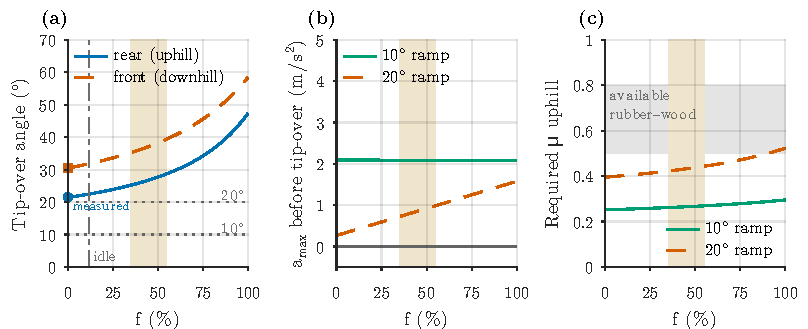
\includegraphics{figures/fig_rampa.pdf}
  \caption{Weight relief on the ramp versus the module weight fraction supported by the rotors, $f$ ($f=0.5$ corresponds to about \SI{1540}{\micro\second} collective). (a) Static backward (uphill forward) and forward (downhill forward) tip-over slopes; dots show the slopes measured on 23 November with the module locked. (b) Tip-over-free acceleration margin at \SI{10}{\degree} and \SI{20}{\degree}, with the full module inertia \eqref{eq:amaxf}. (c) Friction coefficient required at the driven wheels while climbing, with the rubber-on-wood band. The ochre band marks the proposed ramp-mode window.}
  \label{fig:rampa}
\end{figure}

\paragraph{3. Trade-off versus a gimbal}
An honest comparison with a lightweight gimbal is as follows. Under the same model, a \SI{1}{\kilo\gram} motorized gimbal at the same height would achieve a \SI{33.3}{\degree} uphill tip-over slope at zero power cost; the octocopter surpasses it only for $f>0.72$. The drone's advantage is therefore not low mass, but \emph{adjustable} ballast: at $f=0$ it loads the driven wheels for traction, at $f\approx0.5$ it balances tip-over and traction, and at $f=1$ its weight disappears from the base. A gimbal is fixed ballast. Moreover, the octocopter is the project's object of study: an inverted pendulum with actuator delay and limited torque authority validated here, captive and instrumented, prior to free flight. The cost is twofold: power (Section~\ref{sec:bateria}) and a 0.2--\SI{0.3}{\hertz} band in which the octocopter amplifies base accelerations (Section~\ref{sec:coupling}), which base reference ramps must avoid.

\paragraph{What was tested and what remains}
The \SI{10}{\degree} ramp runs on 18 November used the bench firmware with collective at \SI{1300}{\micro\second} ($f\approx0.12$): the drone leveled the tray while providing minimal weight relief. Weight relief is thus still a model prediction. Validating it requires three measurements: base motor current via clamp meter, the duty cycle required to climb at constant speed at $f=0$ and $f=0.5$, and the angle at which the omnidirectional wheels begin to lift on a variable-slope ramp.

\subsection{Thrust margin and endurance versus battery voltage}
\label{sec:bateria}

On 20 November, the module lifted off with the LiPo packs at 12.4\,V at rest, and later failed to lift off at 11.1\,V. This section explains that observation and calculates thrust margin and endurance.

\paragraph{Model}
Each ESC applies a fraction of its branch voltage, $V_{\mathrm{bus}}$, to the motor. With the propeller as load, rotor speed scales with voltage and thrust with its square, so at a fixed command,
\begin{equation}
  T=8k_F'\Big(\frac{V_{\mathrm{bus}}}{V_{\mathrm{ref}}}\Big)^2\Big(\frac{u-u_0}{860}\Big)^n ,
  \label{eq:tv}
\end{equation}
where $k_F'$ is the gain identified at voltage $V_{\mathrm{ref}}$ in Section~\ref{sec:ident}. The branch voltage equals the LiPo open-circuit voltage, $V_{oc}$, minus the drop across internal resistance, the \SI{1}{\metre} cable, and contacts (fuse, relay, XT60), $R_\Sigma$. Because hover power $P_b$ per branch is fixed (thrust equals weight), branch current is $I_b=P_b/V_{\mathrm{bus}}$, and
\begin{equation}
  V_{\mathrm{bus}}=\tfrac12\Big(V_{oc}+\sqrt{V_{oc}^2-4R_\Sigma P_b}\Big).
  \label{eq:vbus}
\end{equation}
Equating \eqref{eq:tv} to weight gives the liftoff collective at another voltage:
\begin{equation}
  u_{\mathrm{req}}=u_0+860\,x_{\mathrm{ref}}\Big(\frac{V_{\mathrm{bus,ref}}}{V_{\mathrm{bus}}}\Big)^{2/n},\qquad x_{\mathrm{ref}}=\frac{u_{\mathrm{ref}}-u_0}{860}=0.68\text{--}0.74,
  \label{eq:ureq}
\end{equation}
and with $n=1.6$ the collective grows as the $1.25$ power of the relative voltage drop. Inputs are: $P_b=\SI{250}{\watt}$ (A2212 with 9450 propeller table from the power audit, \SI{4.2}{\ampere} at 370\,gf and 11.1\,V, scaled as $T^{3/2}$ to 441\,gf per motor); $R_\Sigma=3r_c+\SI{22.6}{\milli\ohm}$, with $r_c=6$--\SI{15}{\milli\ohm} per cell [E] and a 50\% increase below 40\% state of charge; and a typical LiPo rest-voltage versus state-of-charge curve [E]. Result bands combine the extreme values of $k_F'$ and $r_c$.

\paragraph{Results}
Figure~\ref{fig:bateria} and Table~\ref{tab:bateria} give the liftoff collective and available thrust-to-weight ratio versus rest voltage:
\begin{itemize}
  \item At 12.4\,V (93\% charge), each branch delivers \SI{22}{\ampere} at \SI{11.2}{\volt}. The module lifts off at 1725--\SI{1775}{\micro\second}: the firmware \texttt{flotar} (hover) command (\SI{1750}{\micro\second}) falls squarely inside this band. At the \SI{1850}{\micro\second} sustained limit, the thrust-to-weight ratio is 1.20--1.36, and at the \SI{1950}{\micro\second} maximum, 1.48--1.68.
  \item At 11.1\,V at rest (12\% charge), bus voltage drops to \SI{9.3}{\volt} at \SI{27}{\ampere}, and liftoff demands 1850--\SI{2000}{\micro\second}: in the best case right at the sustained limit with no margin for attitude control, and in the worst case beyond what the ESC can deliver. This matches the experimental observation.
  \item The minimum rest voltage for liftoff without exceeding \SI{1850}{\micro\second} is 11.1--\SI{11.6}{\volt} (12--60\% charge). With the fixed \texttt{flotar} command, the module lifts off only above 12.05--\SI{12.1}{\volt}, and at the pessimistic bound of $k_F'$ it never lifts off.
  \item \textbf{Endurance.} Starting from 12.4\,V, continuous hover lasts 2.7--\SI{6.8}{\minute} until liftoff requires \SI{1850}{\micro\second} (3.3--\SI{7.4}{\minute} from 12.6\,V). The energy limit at 80\% discharge would be \SI{6.6}{\minute}. Flight time is therefore limited by thrust margin rather than battery capacity: only the upper end of the discharge curve is usable.
\end{itemize}

\begin{table}[!htbp]
\centering
\caption{Thrust margin versus LiPo voltage at rest (model \eqref{eq:vbus}--\eqref{eq:ureq}). Nominal collective computed with $u_{\mathrm{ref}}=\SI{1750}{\micro\second}$ and $r_c=\SI{10}{\milli\ohm}$; uncertainty band in parentheses.}
\label{tab:bateria}
\footnotesize
\setlength{\tabcolsep}{4pt}
\begin{tabular}{@{}cccccc@{}}
\toprule
$V_{oc}$ (V) & Charge (\%) & $V_{\mathrm{bus}}$ (V) & $I_b$ (A) & $u_{\mathrm{req}}$ (\si{\micro\second}) & Thrust/weight at \SI{1850}{\micro\second} \\
\midrule
12.6 & 100 & 11.45 & 21.8 & 1735 (1710--1760) & 1.24--1.42 \\
12.4 & 93 & 11.23 & 22.3 & 1750 (1725--1775) & 1.20--1.36 \\
12.2 & 84 & 11.00 & 22.7 & 1766 (1739--1793) & 1.14--1.31 \\
12.0 & 78 & 10.78 & 23.2 & 1782 (1754--1811) & 1.09--1.26 \\
11.8 & 68 & 10.55 & 23.7 & 1799 (1769--1831) & 1.04--1.21 \\
11.6 & 59 & 10.33 & 24.2 & 1817 (1786--1852) & 1.00--1.16 \\
11.4 & 40 & 10.10 & 24.8 & 1837 (1803--1875) & 0.95--1.12 \\
11.1 & 12 & 9.32 & 26.8 & 1910 (1850--2000) & 0.74--1.00 \\
\bottomrule
\end{tabular}
\end{table}

\begin{figure}[!htbp]
  \centering
  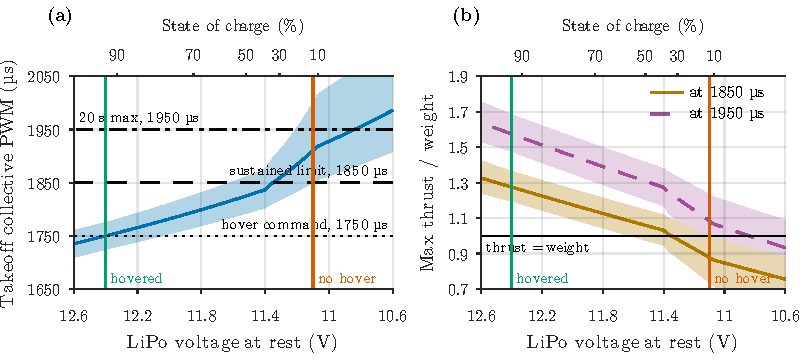
\includegraphics{figures/fig_bateria.pdf}
  \caption{Thrust margin versus LiPo voltage at rest. (a) Liftoff collective \eqref{eq:ureq}: nominal curve and band from uncertainty in $k_F'$ and internal resistance; horizontal lines show the \texttt{flotar} command, sustained limit, and maximum command of firmware v11; top axis shows state of charge. (b) Available thrust-to-weight ratio at the sustained limit and at maximum collective.}
  \label{fig:bateria}
\end{figure}

\paragraph{Comparison with flight logs}
Integrating the logged motor commands from Flights~6--9 on 20 November with the same power model gives a charge draw per battery of 0.10, 0.22, 0.25, and \SI{0.44}{\ampere\hour} (\SI{1.0}{\ampere\hour} total, 31\% of capacity). From this draw, \eqref{eq:ureq} predicts that Flight~9 liftoff required \SI{1787}{\micro\second} (band 1758--\SI{1817}{\micro\second}); the log shows liftoff at \SI{1796}{\micro\second}, compared to \SI{1775}{\micro\second} in Flight~8. At the end of Flight~9 the model predicts roughly 11.6\,V at rest, right on the edge of the sustained limit. The 11.1\,V reading reflects greater discharge than logged: subsequent unlogged attempts, or a measurement taken under load or shortly after landing before LiPo recovery. For this reason, the operating procedure (Section~\ref{sec:operation}) specifies measuring and logging battery voltage at rest.

\paragraph{Design implications}
(i) The firmware should sample VBAT\_A and VBAT\_B (dividers are already wired to GPIO34/35; the power audit recommends changing R2 and R4 to \SI{2.2}{\kilo\ohm} to remain in the ADC linear region below \SI{2.45}{\volt}) and compensate collective via \eqref{eq:ureq} as feedforward, so that \texttt{flotar} means thrust equal to weight rather than a fixed pulse width. (ii) Sessions should be aborted once liftoff exceeds \SI{1825}{\micro\second} to preserve torque margin. (iii) The team's four LiPo packs enable two 3--\SI{7}{\minute} sessions of continuous hover; ramp mode (Section~\ref{sec:porquedron}) draws far less (2--5\% charge per minute) and fits well within that endurance. (iv) Upgrading to 12\,AWG cable cuts cable drop from \SI{0.34}{\volt} to roughly \SI{0.2}{\volt}, saving about \SI{10}{\micro\second} of collective.
